\documentclass[10pt,a4paper]{article}
\usepackage[a4paper,margin=2.3cm]{geometry}
\usepackage[T1]{fontenc}
\usepackage{amsmath,amsthm}
\usepackage{newtxtext,newtxmath}
\usepackage{booktabs}
\usepackage{graphicx}
\usepackage{xcolor}
\usepackage[colorlinks=true,linkcolor=blue!50!black,urlcolor=blue!50!black,citecolor=blue!50!black]{hyperref}
\usepackage{microtype}
\newtheorem{proposition}{Proposition}
\newcommand{\numFailSZero}{18.0}
\newcommand{\numFailSOne}{28.8}
\newcommand{\numFailSTwo}{24.6}
\newcommand{\numErrSZero}{4.8}
\newcommand{\numErrSOne}{6.2}
\newcommand{\numErrSTwo}{8.3}
\newcommand{\numErrSingle}{5.5}
\newcommand{\numErrGB}{5.1}
\newcommand{\numEceSZero}{0.018}
\newcommand{\numEceSOne}{0.025}
\newcommand{\numEceSTwo}{0.070}
\newcommand{\numMIRatioOne}{1.9}
\newcommand{\numMIRatioTwo}{0.90}
\newcommand{\numFlaky}{6.2}
\newcommand{\numBayesErr}{1.2}
\newcommand{\numAurocAleFlaky}{0.92}
\newcommand{\numAurocMIFlaky}{0.91}
\newcommand{\numCovSZero}{90.5}
\newcommand{\numCovSOne}{84.9}
\newcommand{\numCovSTwo}{83.7}
\newcommand{\numRhoMargin}{-0.64}
\newcommand{\numRhoWidth}{0.46}
\newcommand{\numNTotal}{23,000}
\newcommand{\numNReps}{60,000}
\newcommand{\numAutoConf}{90.8}
\newcommand{\numRiskConf}{0.98}
\newcommand{\numRiskOneConf}{1.64}
\newcommand{\numRiskTwoConf}{4.65}
\newcommand{\numRecalOneConf}{0.94}
\newcommand{\numRecalTwoConf}{0.98}
\newcommand{\numAutoRecalOneConf}{79.7}
\newcommand{\numAutoRecalTwoConf}{70.2}
\newcommand{\numAurocZeroConf}{0.940}
\newcommand{\numAurocOneConf}{0.923}
\newcommand{\numAurocTwoConf}{0.894}
\newcommand{\numAutoMI}{90.3}
\newcommand{\numRiskMI}{0.97}
\newcommand{\numRiskOneMI}{1.39}
\newcommand{\numRiskTwoMI}{4.61}
\newcommand{\numRecalOneMI}{0.97}
\newcommand{\numRecalTwoMI}{0.98}
\newcommand{\numAutoRecalOneMI}{78.3}
\newcommand{\numAutoRecalTwoMI}{70.1}
\newcommand{\numAurocZeroMI}{0.931}
\newcommand{\numAurocOneMI}{0.910}
\newcommand{\numAurocTwoMI}{0.891}
\newcommand{\numAutoStack}{89.7}
\newcommand{\numRiskStack}{0.97}
\newcommand{\numRiskOneStack}{0.93}
\newcommand{\numRiskTwoStack}{4.29}
\newcommand{\numRecalOneStack}{0.92}
\newcommand{\numRecalTwoStack}{1.00}
\newcommand{\numAutoRecalOneStack}{81.2}
\newcommand{\numAutoRecalTwoStack}{69.8}
\newcommand{\numAurocZeroStack}{0.939}
\newcommand{\numAurocOneStack}{0.927}
\newcommand{\numAurocTwoStack}{0.890}
\newcommand{\numAutoDis}{87.3}
\newcommand{\numRiskDis}{0.98}
\newcommand{\numRiskOneDis}{0.81}
\newcommand{\numRiskTwoDis}{4.22}
\newcommand{\numRecalOneDis}{0.90}
\newcommand{\numRecalTwoDis}{0.96}
\newcommand{\numAutoRecalOneDis}{76.5}
\newcommand{\numAutoRecalTwoDis}{63.8}
\newcommand{\numAurocZeroDis}{0.921}
\newcommand{\numAurocOneDis}{0.886}
\newcommand{\numAurocTwoDis}{0.862}
\newcommand{\numAutoNov}{45.4}
\newcommand{\numRiskNov}{0.98}
\newcommand{\numRiskOneNov}{0.02}
\newcommand{\numRiskTwoNov}{2.98}
\newcommand{\numRecalOneNov}{0.95}
\newcommand{\numRecalTwoNov}{1.01}
\newcommand{\numAutoRecalOneNov}{25.3}
\newcommand{\numAutoRecalTwoNov}{16.9}
\newcommand{\numAurocZeroNov}{0.490}
\newcommand{\numAurocOneNov}{0.517}
\newcommand{\numAurocTwoNov}{0.533}
\newcommand{\numBudRandZero}{19}
\newcommand{\numBudConfZero}{94}
\newcommand{\numBudCostZero}{94}
\newcommand{\numBudStackZero}{94}
\newcommand{\numBudRandOne}{17}
\newcommand{\numBudConfOne}{82}
\newcommand{\numBudCostOne}{88}
\newcommand{\numBudStackOne}{85}
\newcommand{\numAuditDetect}{90}
\newcommand{\numAuditFalse}{4.8}
\newcommand{\numAuditDetectTwoHundred}{61}

\makeatletter\newcommand{\tabinput}[1]{\@@input #1 }\makeatother

\title{When Can a Learned Test Oracle Be Trusted?\\[2pt]
\large Uncertainty-Guided Acceptance of Verdicts for an Automated Driving Function}
\author{Xiangyu Luo\\[2pt]\small Independent technical study, October 2026\\
\small Code and data: \url{https://github.com/TeamFan/uncertainty-aware-test-oracles}}
\date{}

\begin{document}
\maketitle

\begin{abstract}
\noindent
AI models are increasingly used to judge test outcomes of autonomous cyber-physical systems (ACPS), but an AI verdict is only useful if one knows when to accept it and when to execute the test instead. This study treats that question as a risk-controlled decision. A learned oracle (an ensemble of neural networks) predicts the safety verdict of test cases for a simulated adaptive cruise control with emergency braking, and five uncertainty scores decide which verdicts are accepted. Over \numNTotal{} simulated executions, I find that (i)~for binary verdicts the usual single-pass scores (maximum softmax probability, entropy, Gini impurity, margin) induce identical rankings, so differences must come from multi-inference or external evidence; (ii)~conformal risk control keeps the expected number of accepted false passes per test case at the 1\% target on the nominal operational domain while accepting about \numAutoConf\% of verdicts, but confidence-based acceptance exceeds the target under a shift to low-friction roads and slower sensing (\numRiskOneConf\%), while a stacked error predictor stays within it (\numRiskOneStack\%); (iii)~after a software update of the system under test, all five acceptance rules calibrated on the nominal domain exceed the 1\% target (\numRiskTwoNov--\numRiskTwoConf\% false passes per test case), whereas a random audit of 400 executions detects the update with an estimated \numAuditDetect\% power; and (iv)~spending a 20\% simulation budget on the verdicts with the highest estimated expected cost removes \numBudCostZero\% of the misjudgement cost, against \numBudRandZero\% for random re-execution.
\end{abstract}

\section{Motivation and questions}
Testing an ACPS requires a \emph{test oracle}: a mechanism that decides whether an execution satisfies its requirements~\cite{barr2015}. Learned and foundation models are now proposed as oracles, for example vision-language models that judge robot executions from video~\cite{visor2026}, or as surrogates that predict a test outcome without running a costly simulation. Their verdicts are cheap but fallible, and recent work reports that the uncertainty these models express correlates only weakly with whether they are right~\cite{visor2026}. A test engineer therefore needs an explicit rule: \emph{which AI verdicts can be accepted, and which tests must be executed?}

This study answers four questions on a controlled testbed where the correct verdict of every test case can be obtained by simulation:
\begin{enumerate}
  \item[\textbf{Q1}] Which uncertainty signals identify wrong verdicts, and what do multi-inference signals add to single-pass confidence?
  \item[\textbf{Q2}] Can an acceptance threshold bound the rate of \emph{false passes} (failing executions judged as passing), and does the bound survive a shift of the operational design domain (ODD) or an update of the system under test?
  \item[\textbf{Q3}] Given a limited simulation budget, which verdicts should be re-executed?
  \item[\textbf{Q4}] How does verdict uncertainty relate to non-functional properties of the execution and to the distance from the requirement boundary?
\end{enumerate}

\section{System under test, test cases and shifts}
\paragraph{System under test.} A vectorised longitudinal simulator (time step 0.05\,s, horizon 20\,s) models an adaptive cruise control (ACC) with an automatic emergency braking (AEB) override. The ACC tracks a gap $d^\star=5+h\,v$ with gains on gap error and relative speed; AEB requests $-9\,\mathrm{m/s^2}$ when the measured time-to-collision drops below a trigger value. Braking is limited by road friction $\mu g$ and passes through a 0.25\,s actuator lag. Perception is delayed by a latency, corrupted by Gaussian noise, and loses measurements at a dropout rate (the last value is held).

\paragraph{Test cases and requirement.} A test case fixes eleven parameters: scenario type (lead braking or cut-in), ego and lead speeds, initial gap, braking onset, requested deceleration and final speed of the lead, friction, sensor noise, latency and dropout. The safety requirement is a minimum gap of 2\,m; an execution \emph{fails} if it is violated (collisions included). The behaviour of the other road user is not fully controlled by a test: its deceleration varies by $\pm15\%$ and its braking onset by a 0.3\,s standard deviation between executions. Together with sensor noise, this makes the verdict of a single execution random. Re-executing 3,000 nominal test cases 20 times shows that \numFlaky\% of them are \emph{flaky} (both verdicts observed); averaging $\min(\hat p,1-\hat p)$ over these test cases, with $\hat p$ the observed failure frequency, gives an empirical estimate of the irreducible classification error of \numBayesErr\% (a plug-in estimate from 20 executions per test case).

\paragraph{Data sets.} The nominal ODD (S0) draws the parameters uniformly from engineering ranges (friction 0.6--1.0, latency 0--0.3\,s); \numFailSZero\% of executions fail. Two shifts are studied:
\textbf{S1}, an ODD shift to wet or snowy roads (friction 0.3--0.6) and slower sensing (latency 0.2--0.5\,s), with \numFailSOne\% failures; and
\textbf{S2}, a software update of the SUT (headway 1.5$\to$1.2\,s, softer relative-speed gain, AEB trigger 1.6$\to$1.25\,s) evaluated on nominal test cases, with \numFailSTwo\% failures. S2 leaves the input distribution unchanged and alters only the mapping from test case to verdict. Each test case is executed once to obtain its label: 4,000 for training, 3,000 for fitting auxiliary models, 6,000 nominal test cases for calibration and testing, and 5,000 each for S1 and S2.

\section{Learned oracles and uncertainty signals}
The oracle is a deep ensemble of five multilayer perceptrons (two hidden layers of 64 units), each trained on a bootstrap resample; its verdict is \emph{fail} when the mean probability $\bar p>1/2$. The inputs are the test parameters plus the initial time headway and a kinematic stopping margin, which a test engineer would supply. A second ensemble of five gradient-boosted tree classifiers provides an independent model family. On S0 the ensemble misjudges \numErrSZero\% of executions, against \numErrSingle\% for a single network and \numErrGB\% for the tree ensemble; its expected calibration error is \numEceSZero.

Every score below is oriented so that larger means less trustworthy.
\begin{itemize}\setlength\itemsep{1pt}
  \item \textbf{Confidence}: binary entropy of $\bar p$ (single-pass in form, computed from the ensemble mean).
  \item \textbf{Ensemble mutual information} (epistemic part): $\mathrm{MI}=H[\bar p]-\tfrac{1}{M}\sum_m H[p_m]$; the subtracted term is the expected (aleatoric) entropy.
  \item \textbf{Cross-family disagreement}: $|\bar p-\bar p_{\mathrm{GB}}|$, the analogue of asking a second model.
  \item \textbf{Input novelty}: mean distance to the 10 nearest training test cases in standardised features.
  \item \textbf{Stacked error predictor}: a logistic regression on the logarithms of the four scores above, fitted to the oracle's errors on the separate fitting set.
\end{itemize}

\begin{proposition}
For a binary verdict with probability $p$, the scores $1-\max(p,1-p)$, the binary entropy $h(p)$, the Gini impurity $1-p^2-(1-p)^2$ and the negative margin $-|2p-1|$ are strictly decreasing functions of $|p-\tfrac12|$. Hence they rank test cases identically, and any rank-based evaluation (AUROC, risk--coverage curves, threshold rules on quantiles) gives the same result for all four.
\end{proposition}
\begin{proof}
With $d=|p-\tfrac12|\in[0,\tfrac12]$: $1-\max(p,1-p)=\tfrac12-d$, Gini $=\tfrac12-2d^2$, $-|2p-1|=-2d$, and $h(\tfrac12+d)$ is symmetric in $d$ with derivative $\log\frac{1/2-d}{1/2+d}<0$ for $d>0$.
\end{proof}
The test suite checks this property numerically. Comparing these scores for binary oracles therefore adds no information; with more than two classes (for example the quality levels of~\cite{visor2026}) they differ.

\section{Accepting verdicts with a risk guarantee}
For a threshold $\tau$, the verdict of test case $i$ is accepted when its score $u_i\le\tau$; otherwise the test is executed. The loss $L_i(\tau)=\mathbf 1\{u_i\le\tau\}\,\mathbf 1\{\text{verdict pass},\ \text{execution fails}\}$ counts accepted false passes and is non-decreasing in $\tau$. Conformal risk control~\cite{crc2024} chooses
\[
\hat\tau=\max\Bigl\{\tau:\ \tfrac{n}{n+1}\widehat R_n(\tau)+\tfrac{1}{n+1}\le\alpha\Bigr\},\qquad \widehat R_n(\tau)=\tfrac1n\textstyle\sum_{i=1}^n L_i(\tau),
\]
on $n$ labelled calibration executions, which guarantees $\mathbb E[L_{n+1}(\hat\tau)]\le\alpha$ when calibration and test cases are exchangeable. The target is $\alpha=1\%$ false passes per test case; $n=2{,}000$ nominal executions are drawn at random from the S0 pool, and the procedure is repeated over 200 random calibration/test splits. Under S1 and S2 the nominal threshold is applied unchanged and, alternatively, recalibrated on 300 labelled executions from the shifted set.

For budgeted verification, the misjudgement cost is 10 per false pass and 1 per false fail. With probabilities $\tilde p$ recalibrated by isotonic regression on the fitting set, the expected cost of accepting a verdict is $10\,\tilde p$ for a \emph{pass} and $1-\tilde p$ for a \emph{fail}. With unit execution cost, executing the $B$ verdicts of highest estimated expected cost minimises the estimated expected residual cost under the fitted probabilities; it minimises the true expected cost only if $\tilde p(x)=\Pr(\text{fail}\mid x)$ for every test case, which marginal calibration alone does not ensure.

\section{Results}
\paragraph{Q1: detecting wrong verdicts.}
Table~\ref{tab:auroc} reports how well each score separates wrong from correct verdicts. Confidence, mutual information and the stacked predictor reach AUROC 0.93--0.94 on S0. Input novelty is uninformative (AUROC \numAurocZeroNov): in this domain the oracle errs near the requirement boundary, not in sparsely sampled regions. Detection degrades under both shifts, most under the software update (\numAurocTwoConf{} for confidence). Mean mutual information rises by a factor of \numMIRatioOne{} under the ODD shift but stays at \numMIRatioTwo{} times its nominal value after the software update: \emph{a frozen oracle's uncertainty describes its inputs, not the system that produced the labels}. The expected entropy (aleatoric part) and the mutual information flag flaky test cases almost equally well (AUROC \numAurocAleFlaky{} and \numAurocMIFlaky), so with single-execution labels the decomposition does not separate SUT randomness from model disagreement.

\begin{table}[t]
\centering\small
\caption{AUROC for detecting wrong verdicts (95\% bootstrap intervals, 1,000 resamples). $^\ast$Verdicts of one network; all other rows score the ensemble verdict.}
\label{tab:auroc}
\begin{tabular}{lccc}
\toprule
Score & S0 nominal & S1 ODD shift & S2 software update\\
\midrule
\tabinput{tables/e1.tex}
\bottomrule
\end{tabular}
\end{table}

\begin{figure}[t]
\centering
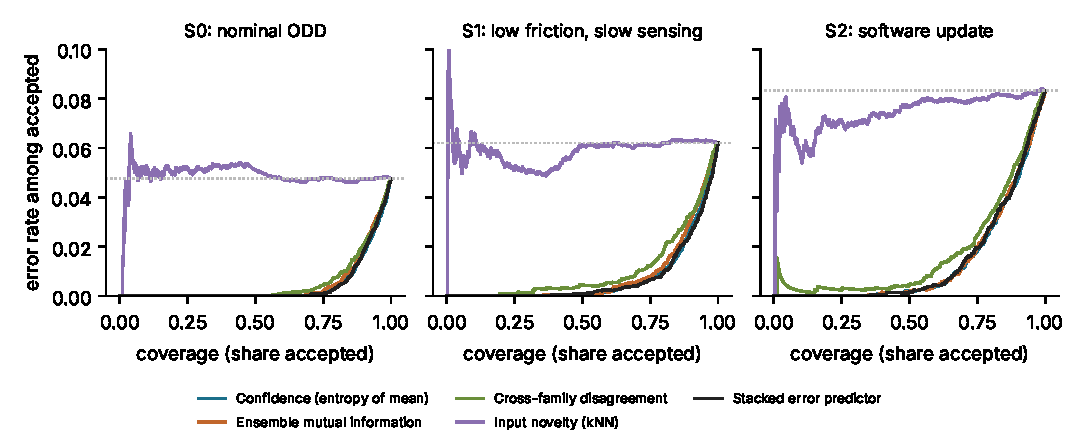
\includegraphics[width=\linewidth]{figures/risk_coverage.pdf}
\caption{Risk--coverage curves: verdicts are accepted from the most to the least certain. The dotted line is the error rate when all verdicts are accepted.}
\label{fig:rc}
\end{figure}

\paragraph{Q2: risk-controlled acceptance.}
Table~\ref{tab:crc} and Figure~\ref{fig:crc} summarise the acceptance rule at $\alpha=1\%$. On S0 every score meets the target (0.97--0.98\%), and the informative scores accept 87--91\% of verdicts, leaving roughly one test in ten to be executed. Under the ODD shift, the nominal threshold lets confidence-based acceptance exceed the target (\numRiskOneConf\%) and mutual information as well (\numRiskOneMI\%), while cross-family disagreement and the stacked predictor stay below it (\numRiskOneDis\% and \numRiskOneStack\%). After the software update all five rules exceed the target, by a factor of three to five (\numRiskTwoNov--\numRiskTwoConf\%), although the scores still rank errors well (AUROC up to \numAurocTwoConf): the ranking survives, but the threshold calibrated on the old system no longer controls the risk. Recalibrating on 300 shifted executions restores the guarantee in both cases at the price of automation: about 80\% of verdicts remain accepted under S1 and 70\% under S2.

Because a frozen oracle scoring unchanged inputs cannot see a change of the SUT, the change must be detected from new executions. A one-sided binomial test that compares the error rate of a random audit with the nominal rate (\numErrSZero\%) detects the update with \numAuditDetectTwoHundred\% power from 200 audited executions and \numAuditDetect\% power from 400, at a false-alarm rate of \numAuditFalse\% on the unchanged system.

\begin{table}[t]
\centering\small
\caption{Conformal risk control of false passes at $\alpha=1\%$: realised false passes per test case (\%) and share of verdicts accepted (\%), averaged over 200 calibration splits. ``S0 cal.''\ applies the nominal threshold to the shifted set; ``recal.''\ recalibrates on 300 shifted executions.}
\label{tab:crc}
\setlength{\tabcolsep}{4pt}
\begin{tabular}{lcccccccc}
\toprule
& \multicolumn{2}{c}{S0} & \multicolumn{3}{c}{S1 ODD shift} & \multicolumn{3}{c}{S2 software update}\\
\cmidrule(lr){2-3}\cmidrule(lr){4-6}\cmidrule(lr){7-9}
Score & risk & accepted & S0 cal. & recal. & accepted & S0 cal. & recal. & accepted\\
\midrule
\tabinput{tables/e2.tex}
\bottomrule
\end{tabular}
\end{table}

\begin{figure}[t]
\centering
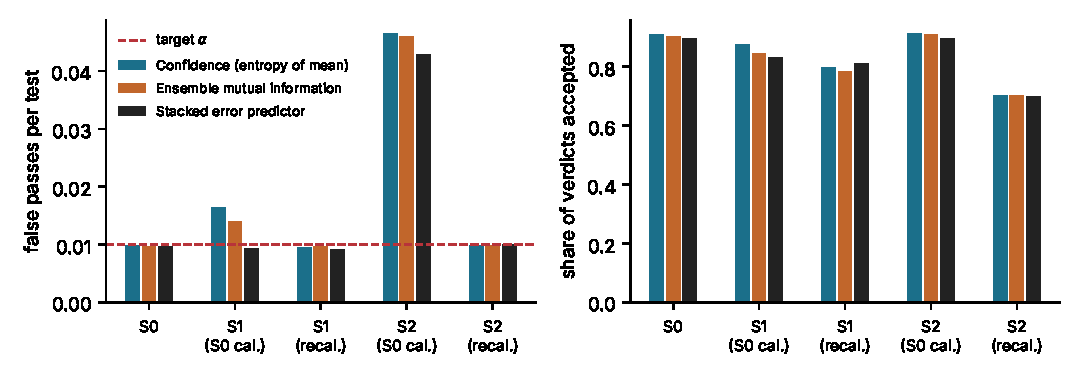
\includegraphics[width=\linewidth]{figures/risk_control.pdf}
\caption{Realised false passes (left) and accepted share (right) for three scores at $\alpha=1\%$.}
\label{fig:crc}
\end{figure}

\paragraph{Q3: spending a simulation budget.}
Figure~\ref{fig:budget} shows the residual misjudgement cost after executing a share of the test cases. Ranking by calibrated expected cost is best at small budgets: with 20\% of tests executed it removes \numBudCostZero\% of the cost on S0 and \numBudCostOne\% on S1, against \numBudRandZero\% and \numBudRandOne\% for random selection and \numBudConfOne\% for confidence ranking on S1. The asymmetric costs matter: the expected-cost rule re-executes uncertain \emph{pass} verdicts before uncertain \emph{fail} verdicts.

\begin{figure}[t]
\centering
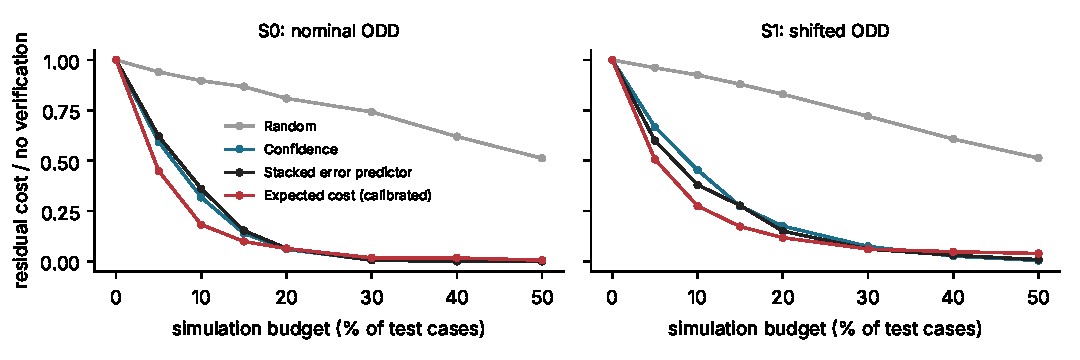
\includegraphics[width=\linewidth]{figures/budget.pdf}
\caption{Residual cost of accepted verdicts (false pass 10, false fail 1) relative to accepting all verdicts.}
\label{fig:budget}
\end{figure}

\paragraph{Q4: non-functional properties and the requirement boundary.}
Verdict uncertainty concentrates on executions close to the requirement boundary (Figure~\ref{fig:margin}; Spearman correlation \numRhoMargin{} between uncertainty and the absolute safety margin). These are also the test cases that discriminate best between correct and faulty behaviour, so deferring uncertain verdicts spends simulation where it is most informative. For the peak deceleration of the ego vehicle, a comfort property, conformalised quantile regression gives 90\% intervals that cover \numCovSZero\% of nominal executions; the coverage falls to \numCovSOne\% under the ODD shift and \numCovSTwo\% after the update, and interval width correlates with verdict uncertainty on S0 (Spearman \numRhoWidth).

\begin{figure}[t]
\centering
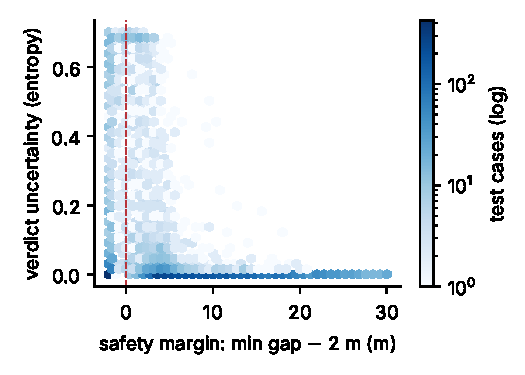
\includegraphics[width=0.52\linewidth]{figures/margin.pdf}
\caption{Verdict uncertainty against the realised safety margin (S0).}
\label{fig:margin}
\end{figure}

\section{Discussion}
Three practical rules follow for using AI verdicts in ACPS testing. First, compare uncertainty scores by the decisions they support, for instance the share of verdicts that can be accepted at a fixed false-pass rate, rather than by correlation alone; for binary verdicts the common single-pass scores are interchangeable. Second, a guarantee obtained on one operational domain needs to be re-established when the domain changes; combining several sources of disagreement made acceptance more robust to an ODD shift in this study. Third, scores that depend only on the test input and are computed by a frozen oracle cannot reveal a change of the system under test when the input distribution is unchanged and no new executions are observed; a risk-based testing process therefore needs a random audit of executions after each software update.

\paragraph{Scope.} The testbed is a longitudinal model with two scenario families, not a full vehicle simulator, and the learned oracle is a tabular classifier rather than a large language or vision-language model. The acceptance rule, the loss and the audit only require a verdict and a score, so the same protocol applies when the verdicts come from a foundation model and the multi-inference signals from repeated sampling or several models, as in~\cite{visor2026,farquhar2024}. Labels come from single executions, so part of the measured error is irreducible (estimated at \numBayesErr\%).

\paragraph{Reproducibility.} \texttt{python scripts/run\_experiments.py} regenerates every number, table and figure in about 40 seconds on two CPU cores (seed 20261028); \texttt{pytest} runs 12 unit tests of the simulator, the scores, the risk-control threshold and the cost model.

\begin{thebibliography}{9}\small
\bibitem{barr2015} E.~T.~Barr, M.~Harman, P.~McMinn, M.~Shahbaz, S.~Yoo. The oracle problem in software testing: a survey. \emph{IEEE Transactions on Software Engineering}, 41(5), 2015.
\bibitem{visor2026} P.~Saurabh, P.~Valle, A.~Arrieta, S.~Ali, P.~Arcaini. VISOR: a vision-language model-based test oracle for testing robots. \emph{AIware}, 2026. arXiv:2605.10408.
\bibitem{crc2024} A.~N.~Angelopoulos, S.~Bates, A.~Fisch, L.~Lei, T.~Schuster. Conformal risk control. \emph{ICLR}, 2024.
\bibitem{farquhar2024} S.~Farquhar, J.~Kossen, L.~Kuhn, Y.~Gal. Detecting hallucinations in large language models using semantic entropy. \emph{Nature}, 630, 2024.
\bibitem{valle2025} P.~Valle, C.~Lu, S.~Ali, A.~Arrieta. Evaluating uncertainty and quality of vision-language-action-enabled robots. arXiv:2507.17049.
\end{thebibliography}
\end{document}
